%%%%%%%%%%%%%%%%%%%%%%%%%%%%%%%%%%%%%%%%%%%%%
\section{Study of the systematic uncertainties}
\label{sec:systematics}
%%%%%%%%%%%%%%%%%%%%%%%%%%%%%%%%%%%%%%%%%%%%%
%We estimate the systematic uncertainty on the post-corrections muon momentum 
%as the linear sum of two contributions accounting for the two common use cases:
The validation procedure described in the previous section is used for
estimating the systematic error on the post-correction momentum of the muons.

There are two common use cases for defining a systematic
error on the momentum scale: 
\begin{itemize}
\item {\sl Case I}: analyses where the spectrum in the data is compared
  with a model known from the simulation. Here the systematic error is
  indicated by the residual
  discrepancy between the the post-correction
  spectrum in the data and in the simulation.
\item {\sl Case II}: analyses aiming to perform an absolute measurement of the
  momentum of the muon, e.g. not relying on a model for the
  expected spectrum. In this case, values of observables built from the measured
  momenta, namely invariant masses, differing from standard
  references are indications of systematic errors. 
\end{itemize}

\underline{\sl Case I}: We define the systematic error  $\Delta p_T$ related to the remaining discrepancy between
the data and the simulation as:
\begin{equation}
  \frac{\Delta p_T}{p_T}=\frac{M_{DATA}-M_{MC}}{M_{DATA}}
  \label{eq:syst_DATA_MC}
\end{equation}
The above relation between momentum
and masses holds under the hypothesis that the systematic errors are fully correlated between the two muons. 
The fractional difference on the mass is shown as a function of $|\eta|$ of one of the two muons in
Figure~\ref{fig:syst_DATA_MC_eta}. 
\begin{figure}[hbtp]  
\begin{center}
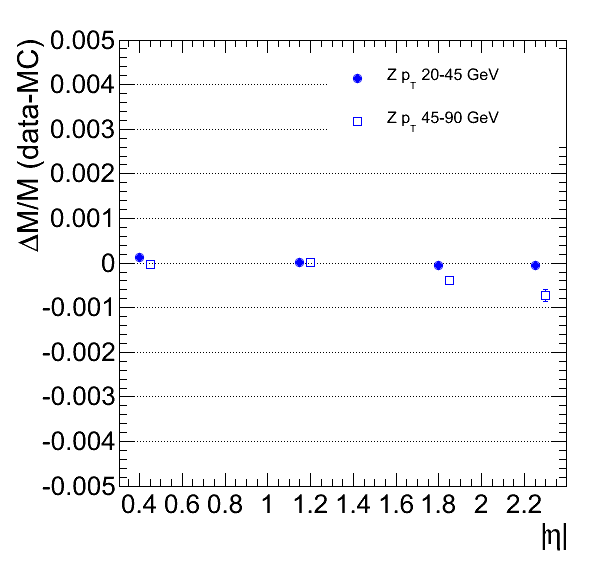
\includegraphics[width=\textwidth]{figures/ScaleEta_afterCorrection}
 \hspace{1cm} 
   \caption{Fractional difference $\frac{M_{DATA}-M_{MC}}{M_{DATA}}$
     for dimuons from Z bosons decays as a function of the $|\eta|$
     of one the two muons (averaged on the second).} 
   \label{fig:syst_DATA_MC_eta} 
 \end{center}
\end{figure} 
The fractional difference is everywhere well within $\pm$0.0010 with the largest value
being around -0.0010, for the point in the large $|\eta|$ and $p_T$ bin.
Conservatively we assign a $\pm$0.0005 uncertainty everywhere apart from this
point where a $\pm$0.0010 uncertainty is assumed. 

\underline{\sl Case II}: The systematic error on $p_T$ has an additional
contribution that we evaluate using the simulation where we take as
estimator the
discrepancy between the values of the mass of the Z boson extracted
from the spectra of the dimuons 
and the world average reported by the Particle Data Group (PDG)~\cite{Beringer:1900zz}:
\begin{equation}
  \frac{\Delta p_T}{p_T}=\frac{M_{MC}-M_{PDG}}{M_{PDG}}
  \label{eq:syst_MC_PDG}
\end{equation}
The above relation between momentum
and masses holds under the hypothesis that the systematic errors are fully correlated between the two muons. 
%Ideally after the calibration procedure, both in
%the simulation and in the data, 
We checked the  behaviour of the fractional mass difference defined
in Eq.~\ref{eq:syst_MC_PDG} against $p_T$ and $|\eta|$ of one of the two
muons using simulated events reconstructed in {\sl realistic} conditions.
Discrepancies from the PDG values, can orginate
from a poor parametrization of the dimuon spectrum
or from biases on the muon momentum not entirely corrected by the
calibration procedure.
% %%%
% realistic conditions -> 
% which should reflect the
% level of knowledge of the calibration and alignment conditions which
% reflects their accuracy in the data. 
% %%%  TO BE DEFINED IN EARLIER  SECTIONS 
Since a not null value of the fractional mass difference will translate directly into the second
contribution of the {\sl Case II} error,
to disentangle the two effects we used a set of
simulated events reconstructed assuming a perfect knowledge of the
calibration and alignment conditions, hereafter referred to as
{\sl ideal} conditions, but with the same set of
dead channels as in real data. Possible biases in the measured momentum due
to approximations in the track reconstruction (e.g. mismodelling
during the reconstruction of the interaction of the charged particle
with the material or with the magnetic field) were the same as
in the standard track reconstruction. In this case no corrections were
applied to the reconstructed muons. 
Details on the samples used for this test are given in Table~\ref{tab:datasets_for_systematics}.
%%%%%%%
\begin{table}[hbH]
\begin{center}
\caption{Datasets \label{tab:datasets_for_systematics}} 
\begin{tabular}{|l|c|c|c|c|}
\hline
Dataset & MC generator & Data-Tier & events & Corrections applied\\
\hline 
DYJetsToLL & MadGraph &  AODSIM              & 2.95 M & MuScleFit \\
DYToMuMu   & POWHEG   &  AODSIM              & 8.60 M & MuScleFit \\
DYToMuMu   & POWHEG   &  START\_53 from RECO & 0.59 M & MuScleFit \\
DYToMuMu   & POWHEG   &  MC\_53 from RECO    & 0.59 M & nocorrections \\
\hline
\hline
\end{tabular}
\end{center}
\end{table}
%%%%
%%%%			
%\begin{figure}[hbtp]  
%\begin{center}
%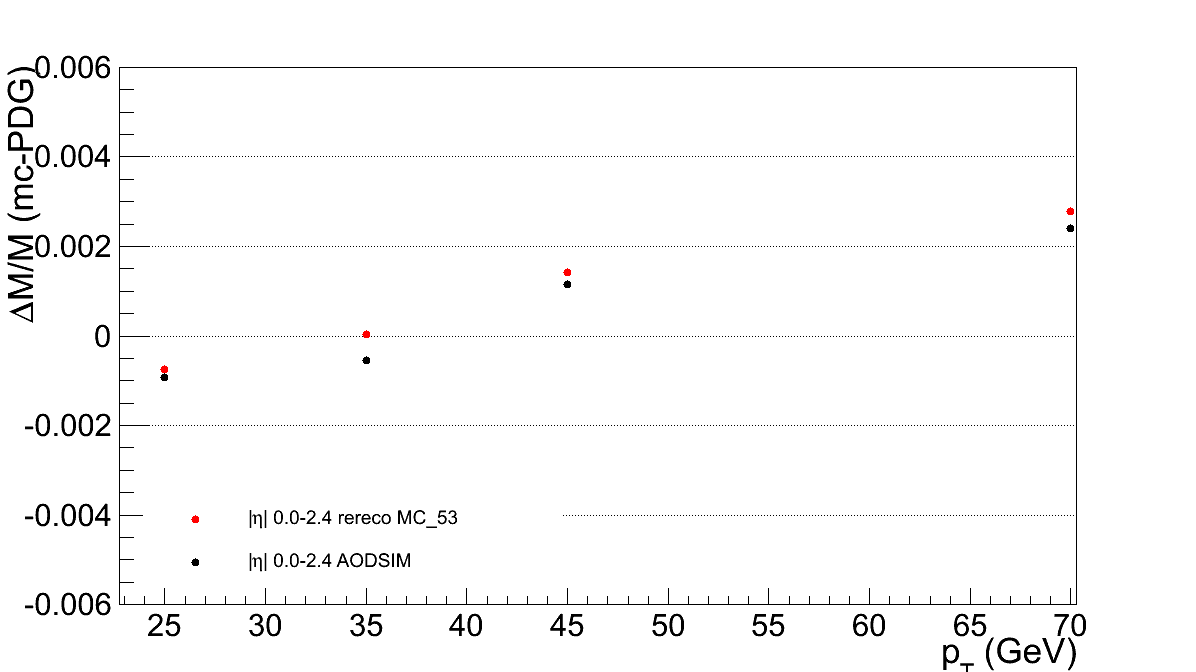
\includegraphics[width=\textwidth]{figures/ScalePdg_mc_Pt_Z}
% \hspace{1cm} 
%   \caption{Fractional difference $\frac{M_{MC}-M_{PDG}}{M_{MC}}$
%     (tbc) for dimuons from Z bosons decays as a function of the $p_T$
%   of one the two muons (averaged on the second).} 
%   \label{fig:syst_MC_PDG_pT} 
% \end{center}
%\end{figure} 
\begin{figure}[hbtp]  
\begin{center}
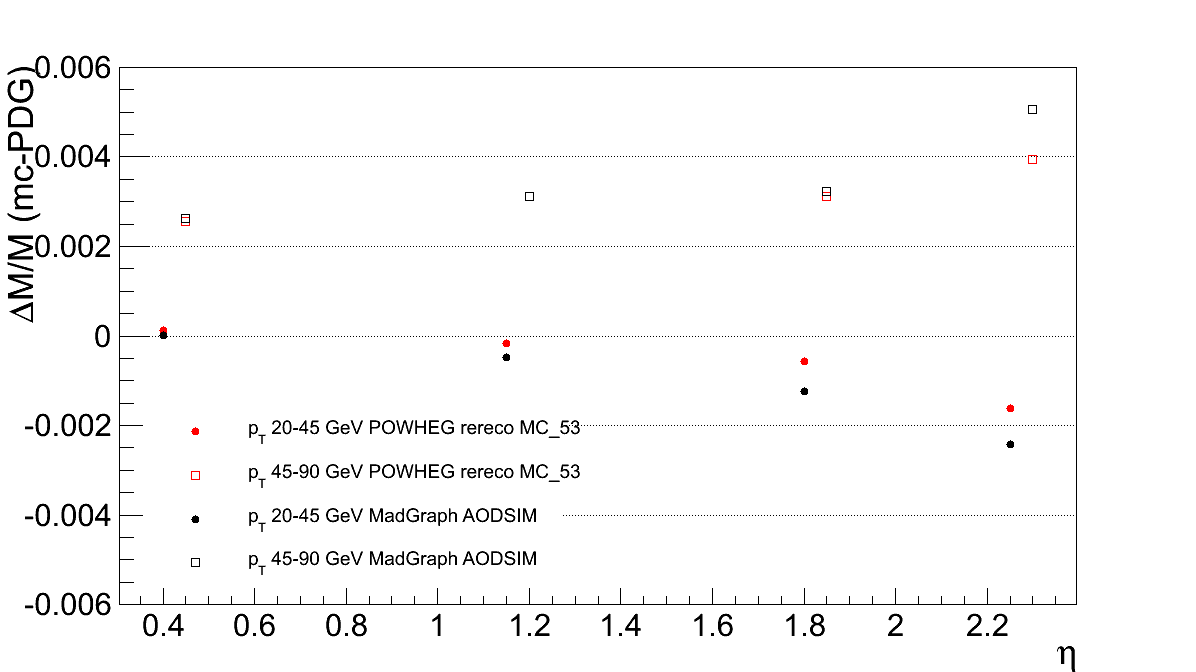
\includegraphics[width=\textwidth]{figures/ScalePdg_mc_Eta_Z}
 \hspace{1cm} 
   \caption{Fractional difference $\frac{M_{MC}-M_{PDG}}{M_{MC}}$
     (tbc) for dimuons from Z bosons decays as a function of the $|\eta|$
   of one the two muons (averaged on the second).} 
   \label{fig:syst_MC_PDG_eta} 
 \end{center}
\end{figure} 
%Figure~\ref{fig:syst_MC_PDG_pT} shows the fractional difference on the
%mass as a function of $p_T$ of one of the
%two muons. Points for realistic simulation (post-correction) show a
%bias increasing with $p_T$. The same trend is observed for the points
%obtained with the ideal simulation which agree the with the others 
%at the 0.0005 level on all the $p_T$ range. 
Figure~\ref{fig:syst_MC_PDG_eta} shows the fractional difference on
the mass as a function of $|\eta|$ of one of the two muons in two
different ranges of $p_T$. For $p_T$ in the range [20,45] GeV, values
form the realistic simulation (post-correction) are about -0.0005
for $|\eta|<$1.5 increasing up to -0.0020 at the largest $|\eta|$.
A similar trend is observed for points from the simulation in ideal
conditions. For $p_T$ in the range [45,90] GeV there is approximately
a +0.0020 bias growing up to +0.0050 at the largest $|\eta|$ bin.

\FIXME quote the checks with GEN level infos

Based on this analysis, the systematic errors estimated for the
different $p_T$ and $|\eta|$ ranges are those summarized in
Table~\ref{tab:systematics}.
%%%%%%%
\begin{table}[hbH]
\begin{center}
\caption{Estimated systematic uncertainties on the momentum scale
  post-correction of muons reconstructed in the data.
  Second column corresponds to {\sl Case I} systematics, while
  the sum of second and third columns corresponds to {\sl Case II}
  systematics described in the text.\label{tab:systematics}} 
\begin{tabular}{|l|c|c|}
\hline
$\frac{\Delta p_T}{p_T}$ & MC - PDG & DATA - MC \\
\hline 
$p_T<$45 GeV,   0$<|\eta|<$1.5 & $\pm$0.0005 & $\pm$0.0005\\
$p_T<$45 GeV, 1.5$<|\eta|<$2.4 & $\pm$0.0020 & $\pm$0.0005\\
$p_T>$45 GeV,   0$<|\eta|<$2.0 & $\pm$0.0030 & $\pm$0.0005\\
$p_T>$45 GeV, 2.0$<|\eta|<$2.4 & $\pm$0.0050 & $\pm$0.0010\\
\hline
\hline
\end{tabular}
\end{center}
\end{table}
%%%%
